%% SW arkitektur: Logical View

Logical View skal danne et overblik over hvilke softwarepakker der befinder sig på vores platforme. Blokkene inde i de respektive pakker kan sammen med domænemodellen hjælpe med at give et overblik over hvilke klasser og kernemoduler der skal bruges.

\begin{figure}[htbp] \centering
{\includegraphics[scale=0.7]{filer/systemarkitektur/logical_view_devkit}}
\caption{Logical view for Devkit8000 illustrerer hvilke softwarepakker der befinder sig på Masteren }
\label{fig:Logical View Devkit8000}
\end{figure}

Figur \ref{fig:Logical View Devkit8000} illustrerer hvilke softwarepakker der ligger på Masteren. I bunden er \textit{Device drivers}-pakken som håndterer SPI kommunikationen imellem Devkit8000 og PSoC. I midten ligger \textit{Hardware API}-pakken som håndterer protokol-vedtægter ifm. kommunikationen. \textit{Application}-pakken tager sig af alt UI samt log og fejlhåndtering.

\clearpage

\newenvironment{figure1}[1][]{\begin{figure}[#1]\vspace{3.0cm}}{\vspace{1.0cm}\end{figure}}
\begin{figure1}[htbp] \centering
{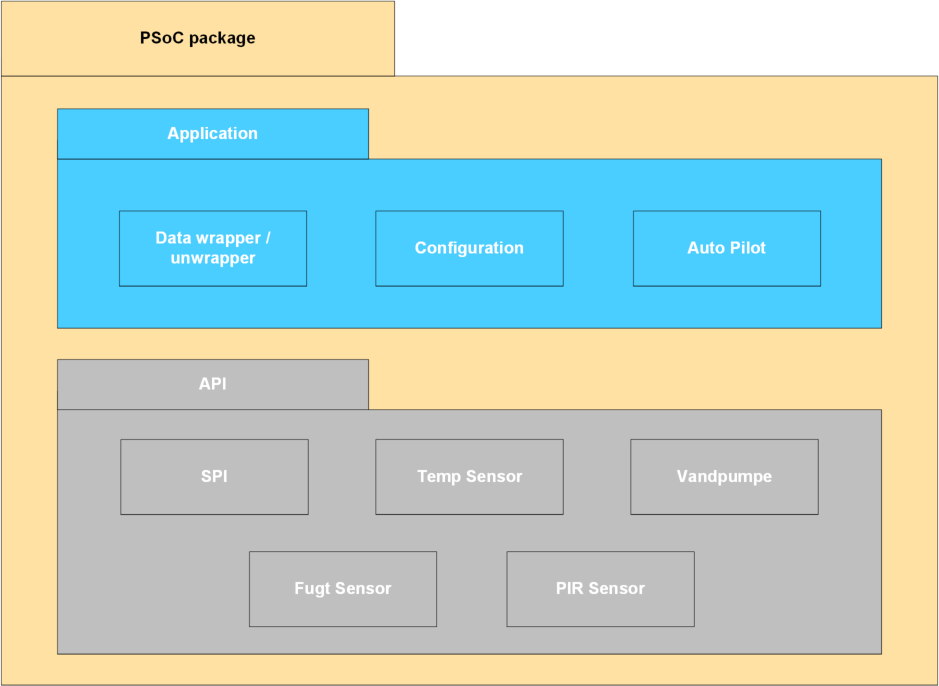
\includegraphics[scale=0.7]{filer/systemarkitektur/logical_view_psoc}}
\caption{Logical view for PSoC illustrer hvilke software pakker der befinder sig på enhederne}
\label{fig:Logical View PSoC}
\end{figure1}

Figur \ref{fig:Logical View PSoC} illustrerer hvilke softwarepakker der ligger på Enhederne. \textit{API}-pakken består af den software som håndterer hardwaren, dvs. den tager imod input og får formateret det til noget brugbart for \textit{Application}-pakken. \textit{Application}-pakken håndterer den indsamlede data som den får fra sensorene igennem \textit{API}-pakken. Denne data sammensættes iht. protokollen og sendes til API pakken som får det sendt til Devkit8000. Pakken skal også håndterer data fra Devkit8000 til at konfigurerer de parametre der styrer automatiseringen af vandingen.

